\chapter{Methods}\label{sec:MM}
\markright{\thechapter~Materials and methods}

\section{Slab configurator}
The computational work presented in this thesis is based on a Python-based design and optimisation framework initiated by the Sustainability in Structural Design Team at kfmResearch \cite{kfmResearch2026}. The original framework provided the general structure for the GWP optimisation of floor system cross-sections across different structural systems and for their environmental performance assessment. Within the scope of this thesis, the framework was further developed by incorporating additional slab systems and implementing the automated handling of non-structural floor build-ups.

The overall workflow is shown schematically in Figure~\ref{fig:slab_configurator_workflow}. The calculation starts with the material and product database. Based on the selected slab system, a cross-section object is created from the available materials and geometric start values. The cross-section is then combined with a member object, which defines the structural system, span, loading and requirements. The member is verified in ULS, SLS 1, SLS 2 and fire according to Table~\ref{Tab: SustFact}. For the structural cross-section a floor build-up is automatically created to satisfy the acoustic insulation requirements against airborne and impact sound. If the selected cross-section does not satisfy the governing requirements, the optimiser modifies selected cross-section parameters until a suitable design is found.  

\begin{figure}[htbp]
\centering
\resizebox{\textwidth}{!}{%
\begin{tikzpicture}[
    font=\scriptsize,
    >=Latex,
    arrow/.style={->, thick},
    note/.style={align=left},
    line/.style={thick}
]

% ------------------------------------------------------------------
% Column x-positions
% ------------------------------------------------------------------
\def\xData{0}
\def\xCS{4.2}
\def\xMember{10.8}

% Titles
\node[font=\bfseries\small] at (\xData,3.6) {Data};
\node[font=\bfseries\small] at (\xCS,3.6) {Cross-section};
\node[font=\bfseries\small] at (\xMember,3.6) {Member};

% ------------------------------------------------------------------
% Data block
% ------------------------------------------------------------------
\node[cylinder, draw, shape border rotate=90, aspect=0.25,
      minimum height=2.0cm, minimum width=1.25cm, align=center] (db) at (\xData,2.1)
      {Materials\\[2pt]CO$_2$ eq/m$^3$\\[2pt]CHF/m$^3$};

\node[note, anchor=north] at (\xData,0.85) {Material\\variations};

% ------------------------------------------------------------------
% Cross-section block
% ------------------------------------------------------------------
\coordinate (cs0) at (3.0,1.85);

\draw[line] (cs0) rectangle ++(2.8,0.85);
\fill[brown!80] ($(cs0)+(0,0)$) rectangle ++(2.8,0.35);
\fill[gray!60] ($(cs0)+(0,0.35)$) rectangle ++(2.8,0.30);
\fill[violet!70] ($(cs0)+(0,0.65)$) rectangle ++(2.8,0.08);
\fill[gray!30] ($(cs0)+(0,0.73)$) rectangle ++(2.8,0.12);

\draw[decorate,decoration={brace,amplitude=4pt}]
    (5.95,2.70) -- (5.95,2.50);

\node[anchor=west,align=left]
    at (6.15,2.80)
    {Automated\\[-4pt]floor build-up};

% Structural cross-section brace
\draw[decorate,decoration={brace,amplitude=4pt}]
    (5.95,2.50) -- (5.95,1.85)
    node[midway,right=6pt]
    {Cross-section};

\node[green!60!black, font=\large] at (8.25,2.1) {$\circlearrowleft$};
%\node[yellow!80!black, font=\large] at (8.15,3) {$\lightning$};

\node[note, anchor=north west] at (3.0,1.35) {Cross-section\\
$\bullet$ Fulfils requirements\\
$\bullet$ Optimised for GWP};

\node[green!60!black, font=\large] at (6.25,0.05) {$\circlearrowleft$};

% ------------------------------------------------------------------
% Member block
% ------------------------------------------------------------------
\coordinate (b1) at (10.0,2.10);
\coordinate (b2) at (12.3,2.10);

% Beam
\draw[line] (b1) -- (b2);

% Distributed load
\draw[red, thick] ($(b1)+(0,0.55)$) -- ($(b2)+(0,0.55)$);
\draw[red, thick] ($(b1)+(0,0.55)$) -- (b1);
\draw[red, thick] ($(b2)+(0,0.55)$) -- (b2);

\foreach \x in {10.0,10.75,11.50,12.3} {
    \draw[red, ->] (\x,2.65) -- (\x,2.25);
}

% Supports
\draw[line] (10.0,2.10) -- ++(-0.16,-0.27) -- ++(0.32,0) -- cycle;
\draw[line] (12.3,2.10) -- ++(-0.16,-0.27) -- ++(0.32,0) -- cycle;

% Span
%\draw[<->] (10.0,1.45) -- (12.3,1.45);
%\node at (11.15,1.22) {$L$};

% Member labels
\node[note, anchor=west] at (12.65,2.55) {Load combination};
\node[note, anchor=west] at (12.65,1.85) {Structural system};

\node[note, anchor=north west] at (10.0,1.35) {Requirements\\
$\bullet$ ULS\\
$\bullet$ SLS 1: Deflection\\
$\bullet$ SLS 2: Vibration\\
$\bullet$ Fire};

% ------------------------------------------------------------------
% Arrows between blocks
% ------------------------------------------------------------------
\draw[arrow] (1.25,2.1) -- (2.25,2.1);
\draw[arrow] (8.55,2.1) -- (9.45,2.1);

\end{tikzpicture}%
}
\caption{Slab configurator workflow from material database to cross-section optimisation and member comparison.}
\label{fig:slab_configurator_workflow}
\end{figure}

The comparison is carried out in two stages. First, each slab system is optimised for the selected design criterion and span. Second, the resulting feasible members are compared according to the identified factors for sustainability, defined in Table~\ref{Tab: SustFact}.

It is noted that the slab configurator is used as a comparative design tool. It does not replace a detailed project-specific structural design, but it enables a consistent assessment of the relative influence of slab system, span, material choice, acoustic build-up and governing design criterion.


\subsection{Material database}
The material database was selected by the Sustainability in Structural Design Team of \textit{kfmResearch} \cite{kfmResearch2026}. It contains mechanical material properties and product-specific environmental data. Environmental Product Declarations (EPDs) are stored on product level and are linked to the mechanical property classes used by the structural models. The database therefore allows a distinction between mechanical performance and producer-specific environmental impact. For concrete, reinforcing steel, prestressing steel, and timber products, the database stores product density, material class and total GWP values. These properties enable the assessment of producer-specific GWP, mass, and structural height, including product-specific variations. As identified in the literature review, GWP, mass, and height are key indicators for the sustainability assessment of floor systems.

The range of product-specific GWP values stored in the database is summarised in Table~\ref{tab:product_specific_gwp_values}. Negative values occur for timber products where biogenic carbon storage is included in the reported GWP. Each product is assigned to a material class, which defines the corresponding mechanical and physical properties listed in Table~\ref{tab:material_properties}.

\begin{table*}[h]
    \centering
    \begingroup
    \scriptsize
    \setlength{\tabcolsep}{3pt}
    \renewcommand{\arraystretch}{1.12}
    \begin{tabularx}{\textwidth}{@{}
        >{\raggedright\arraybackslash}X
        |>{\raggedright\arraybackslash}X
        |c|r|r@{}}
    \hline
    \textbf{Material} &
    \textbf{Material class} &
    \textbf{Products} &
    \textbf{$GWP_{\min}$} &
    \textbf{$GWP_{\max}$} \\
    &
    &
    &
    kg CO$_2$-eq/t &
    kg CO$_2$-eq/t \\
    \hline

    Ready-mixed concrete & C20/25 & 7  & 77.0   & 102.4 \\
    Ready-mixed concrete & C25/30 & 8  & 75.4   & 100.1 \\
    Ready-mixed concrete & C30/37 & 9  & 76.7   & 104.2 \\
    Reinforcing steel    & B500B  & 18 & 352.9  & 922.7 \\
    Prestressing steel   & Y1860  & 9  & 389.0  & 2250.0 \\
    Glue-laminated timber& GL24h  & 21 & -1534.9& 765.5 \\
    Solid structural timber & C24 & 10 & 75.7   & 363.0 \\
    3- and 5-ply wood    & C24    & 13 & -66.2  & 556.0 \\
    3- and 5-ply wood    & GL24h  & 3  & 250.0  & 415.6 \\
    \hline
    \end{tabularx}
    \endgroup
    \caption{Product-specific GWP values used for the sustainability assessment.}
    \label{tab:product_specific_gwp_values}
\end{table*}

\begin{table*}[htbp]
    \centering
    \begingroup
    \scriptsize
    \setlength{\tabcolsep}{3pt}
    \renewcommand{\arraystretch}{1.15}
    \begin{tabularx}{\textwidth}{@{}>{\raggedright\arraybackslash}X|r|r|r|r|r|r|r|r|>{\raggedright\arraybackslash}X|r|r@{}}
    \hline
    \textbf{Class} &
    \textbf{$f_c$} &
    \textbf{$f_t$} &
    \textbf{$f_m$} &
    \textbf{$f_v$} &
    \textbf{$E$} &
    \textbf{$\rho$} &
    \textbf{$\beta_n$} &
    \textbf{$\varphi$} &
    \textbf{Connector type} &
    \textbf{$d$} &
    \textbf{$K_{\mathrm{ser}}$} \\
    &
    MPa &
    MPa &
    MPa &
    MPa &
    GPa &
    kg/m$^3$ &
    mm/min &
    -- &
    -- &
    mm &
    N/m \\
    \hline

    C20/25 &
    20 &
    2.3 &
    -- &
    -- &
    30 &
    2241–2440 &
    -- &
    2.5 &
    -- &
    -- &
    -- \\

    C25/30 &
    25 &
    2.6 &
    -- &
    -- &
    32 &
    2242–2439 &
    -- &
    2.5 &
    -- &
    -- &
    -- \\

    C30/37 &
    30 &
    2.9 &
    -- &
    -- &
    34 &
    2332–2430 &
    -- &
    2.5 &
    -- &
    -- &
    -- \\

    B500B &
    500 &
    500 &
    -- &
    -- &
    205 &
    7850 &
    -- &
    -- &
    -- &
    -- &
    -- \\

    GL24h &
    -- &
    -- &
    24 &
    1.8 &
    11.5 &
    424–483 &
    0.7 &
    0.6 &
    -- &
    -- &
    -- \\

    C16 &
    -- &
    -- &
    16 &
    1.5 &
    8.0 &
    500 &
    0.8 &
    0.6 &
    -- &
    -- &
    -- \\

    C24 &
    -- &
    -- &
    24 &
    1.5 &
    11.0 &
    400–523 &
    0.8 &
    0.6 &
    -- &
    -- &
    -- \\

    Y1860 &
    -- &
    1860 &
    -- &
    -- &
    195 &
    7850 &
    -- &
    -- &
    -- &
    -- &
    -- \\

    DBS\_6 &
    -- &
    -- &
    -- &
    -- &
    -- &
    -- &
    -- &
    -- &
    Screw &
    6 &
    $5.83 \times 10^6$ \\

    DBS\_8 &
    -- &
    -- &
    -- &
    -- &
    -- &
    -- &
    -- &
    -- &
    Screw &
    8 &
    $7.78 \times 10^6$ \\

    DBS\_10 &
    -- &
    -- &
    -- &
    -- &
    -- &
    -- &
    -- &
    -- &
    Screw &
    10 &
    $9.70 \times 10^6$ \\

    DBS\_12 &
    -- &
    -- &
    -- &
    -- &
    -- &
    -- &
    -- &
    -- &
    Screw &
    12 &
    $1.167 \times 10^7$ \\

    Kerve\_20 &
    -- &
    -- &
    -- &
    -- &
    -- &
    -- &
    -- &
    -- &
    Notched &
    -- &
    $1.00 \times 10^9$ \\

    Kerve\_30 &
    -- &
    -- &
    -- &
    -- &
    -- &
    -- &
    -- &
    -- &
    Notched &
    -- &
    $1.50 \times 10^9$ \\

    Two-layer parquet &
    -- &
    -- &
    -- &
    -- &
    -- &
    555 &
    -- &
    -- &
    -- &
    -- &
    -- \\

    Cement screed &
    -- &
    -- &
    -- &
    -- &
    21.0 &
    1850 &
    -- &
    -- &
    -- &
    -- &
    -- \\

    Insulation (glass wool) &
    -- &
    -- &
    -- &
    -- &
    $6\times10^{-6}$ &
    80 &
    -- &
    -- &
    -- &
    -- &
    -- \\
    
    Crushed gravel &
    -- &
    -- &
    -- &
    -- &
    -- &
    2000 &
    -- &
    -- &
    -- &
    -- &
    -- \\

    \hline
    \end{tabularx}
    \endgroup
    \caption{Mechanical properties data on characteristic design level. Mass is stored producer-specific.}
    \label{tab:material_properties}
\end{table*}

During the thesis, the database was extended with material-specific (not producer-specific) cost and construction time as listed in Table~\ref{tab:cost_time_assumptions}. The values are derived from NPK positions, market data, literature sources and engineering estimates.

\begin{table*}[htbp]
    \centering
    \begingroup
    \scriptsize
    \setlength{\tabcolsep}{3pt}
    \renewcommand{\arraystretch}{1.12}
    \begin{tabularx}{\textwidth}{@{}X|c|c|c|c|X@{}}
    \hline
    \textbf{Material / Component} &
    \textbf{Cost} &
    \textbf{Cost unit} &
    \textbf{Time} &
    \textbf{Time unit} &
    \textbf{Reference and description} \\ \hline

    Ready-mixed concrete, formwork &
    75.71 & CHF/m$^2$ & 0.70 & h/m$^2$ &
    NPK 241.261.301, logistics, propping, levelling, oiling and cleaning \cite{CIB19076}.\\

    Ready-mixed concrete, rib. formwork &
    151.42 & CHF/m$^2$ & 1.40 & h/m$^2$ &
    Logistics, propping, levelling, oiling and cleaning \cite{Ammann2024}.\\

    Reinforcing steel &
    2.01 & CHF/kg & 0.009 & h/kg &
    NPK 241.511.123, placing \cite{CIB19076}.\\

    Prestressing steel &
    6.00 & CHF/kg & 0.020 & h/kg &
    Assumed cost and labour input. \\

    Ready-mixed concrete &
    205.29 & CHF/m$^3$ & 0.30 & h/m$^3$ &
    NPK 241.661.112, placing, vibrating, levelling and cleaning \cite{CIB19076}. \\

    Glue-laminated timber &
    1750.00 & CHF/m$^3$ & 1.00 & h/m$^3$ &
    Assumed market price including logistics and connections. \\

    Solid structural timber &
    1250.00 & CHF/m$^3$ & 1.00 & h/m$^3$ &
    NPK 335.531.114, logistics and connections. \\

    DBS 6, Screw TCC conn., d=6 mm &
    5.00 & CHF/piece & 0.010 & h/piece &
    Assumed, logistics and assembly. \\

    DBS 8, Screw TCC conn., d=8 mm &
    5.50 & CHF/piece & 0.010 & h/piece &
    Assumed, logistics and assembly. \\

    DBS 10, Screw TCC conn., d=10 mm &
    6.00 & CHF/piece & 0.015 & h/piece &
    Assumed, logistics and assembly. \\

    DBS 12, Screw TCC conn., d=12 mm &
    6.50 & CHF/piece & 0.015 & h/piece &
    Assumed, logistics and assembly. \\

    Kerve, TCC connector &
    30.00 & CHF/piece & 0.010 & h/piece &
    Assumed, preparation and cleaning. \\

    Two-layer parquet, 11 mm &
    106.00 & CHF/m$^2$ & 0.30 & h/m$^2$ &
    Swiss market price according to \cite{Bodenleger2026}. \\

    Cement screed &
    337.60 & CHF/m$^3$ & 0.15 & h/m$^2$ &
    NPK 661.711.111, labour productivity according to \cite{Steelmonks2026}. \\

    Insulation (glass wool) &
    335.00 & CHF/m$^3$ & 0.10 & h/m$^2$ &
    NPK 661.433.114, acoustic insulation layer. \\

    Crushed gravel &
    253.20 & CHF/m$^3$ & 0.20 & h/m$^2$ &
    NPK 364.921.111, ballast and protection layer. \\ \hline
    \end{tabularx}
    \endgroup
    \caption{Cost and construction-time input data used for the sustainability assessment.}
    \label{tab:cost_time_assumptions}
\end{table*}

\newpage
\subsection{Contribution to the existing Python framework}
Since this thesis is based on an existing Python framework, it is important to highlight the contributions made within its scope. The initial configurator was able to handle solid rectangular concrete, ribbed concrete, solid rectangular timber, and ribbed timber hollow-core cross-sections. The one-dimensional static systems covered were simple-span and continuous beams. For the two-dimensional case, the framework was able to handle line-supported rectangular slabs without continuity over the supports.

\subsubsection{Cross-section handling}
All cross-section classes were updated with respect to the calculation of material quantities, GWP, cost, and construction time. These calculations are now normalised per square metre of floor area and account for quantities that develop in the transverse direction. This enables a consistent comparison between one-dimensional systems with defined tributary widths and two-dimensional slab systems.
Furthermore, all systems were linked to the automated acoustic floor build-up generator described in Section~\ref{Sec: AutFloor}. Following the structural optimisation, the generator determines the lightest floor build-up that satisfies the specified acoustic requirements.
The specific modifications made to the individual cross-section classes are summarised in Table~\ref{tab:existing_system_developments}.

\begin{table*}[h]
    \centering
    \begingroup
    \scriptsize
    \setlength{\tabcolsep}{3pt}
    \renewcommand{\arraystretch}{1.15}
    \begin{tabularx}{\textwidth}{@{}
        >{\raggedright\arraybackslash}p{3.2cm}
        |>{\raggedright\arraybackslash}X
        |>{\raggedright\arraybackslash}X@{}}
    \hline
    \textbf{Cross-section class} &
    \textbf{Further development} &
    \textbf{Effect on the assessment} \\
    \hline

    Ribbed timber hollow-core &
    Internal cavity insulation added to the acoustic model and non-structural mass calculation. &
    Improves the acoustic model of the hollow-core cross-section.\\

    Ribbed reinforced concrete &
    Separate resistance checks introduced for positive span bending and negative support bending.  &
    Extends ULS validation from span moment to support moment.  \\

    Rectangular reinforced concrete &
    Two-way slab analysis extended to include upper support reinforcement in the optimisation for continuous systems. As equal spans are assumed, the optimised reinforcement in the \(x\)-direction is applied in the \(y\)-direction. &
    Enables the optimisation of negative bending reinforcement quantities for continuous systems. \\

    Point-supported reinforced concrete &
    Punching shear calculation of the required punching reinforcement resistance. Required punching reinforcement is converted into an additional steel quantity. &
    Includes the environmental, economic and construction-time effects of punching reinforcement without excluding systems solely based on the need for such reinforcement. \\

    \hline
    \end{tabularx}
    \endgroup
    \caption{Cross-section-specific developments introduced for existing structural systems.}
    \label{tab:existing_system_developments}
\end{table*}

\subsubsection{Static system handling}
The analysis of two-dimensional floor systems was extended to distinguish between line-supported and point-supported structural systems. In addition, continuity over the supports was introduced. Internal forces and deflections were determined in accordance with the existing implementation using:

\begin{equation}
\begin{aligned}
M_d &= \alpha_{M,\mathrm{system}} q_d l^2,\\
V_d &= \alpha_{V,\mathrm{system}} q_d l,\\
w &= \alpha_{w,\mathrm{system}}\frac{q_d l^4}{EI}.
\end{aligned}
\end{equation}

The coefficients $\alpha_{M,\mathrm{system}}$, $\alpha_{V,\mathrm{system}}$, and $\alpha_{w,\mathrm{system}}$ were derived from a finite-element slab analysis performed in Cubus Cedrus. For point-supported systems, the model consisted of a regular $4 \times 4$ column grid subjected to a uniformly distributed load. The columns had a cross-section of $0.25 \times 0.25 \mathrm{m}$. Line-supported systems were represented by walls with a thickness of $0.20\mathrm{m}$ and a height of $0.10\mathrm{m}$. Vertical displacements at the supports were restrained. Bending moments and shear forces were evaluated over an averaged width of one metre within the support strip, whereas deflections were evaluated at mid-span. The coefficients were determined for spans of 3, 5, 6, 7, 8, 10, 12, and 16\,m and subsequently implemented in the configurator through a database storage.

For ULS bending verification of two-dimensional rectangular concrete slabs, plastic moment redistribution was added as an optional modification of the elastic moment coefficients. The elastic coefficients from the slab database remain the basis for the analysis, but they are replaced by redistributed coefficients when the slab system and the cross-section provide sufficient rotational capacity. This redistribution is only applied to reinforced and post-tensioned rectangular concrete slabs. The available ductility classes of the positive and negative bending zones are compared with the required ductility classes stored for the corresponding slab system. If the requirement is not fulfilled, the elastic coefficients are retained. If it is fulfilled, positive span moments are increased and negative support moments are reduced by system-specific factors:

\begin{equation}
\alpha_{M,\mathrm{red},i}
=
\begin{cases}
k_{+}\,\alpha_{M,i}, & \alpha_{M,i} \geq 0,\\
k_{-}\,\alpha_{M,i}, & \alpha_{M,i} < 0.
\end{cases}
\end{equation}

For line-supported continuous slabs, the factors \(k_{+}=1.51\) and \(k_{-}=0.76\) were used. For point-supported continuous slabs, the factors were \(k_{+}=1.47\) and \(k_{-}=0.68\). The redistributed moment coefficients are used only in the ULS bending resistance check; shear, punching shear, deflection and vibration checks remain based on the corresponding elastic coefficients.

\subsection{Timber--concrete composite slab}

Timber--concrete composite (TCC) slabs were modelled as unidirectional structural systems consisting of a timber tension member and a concrete compression layer. Composite action is partially achieved through mechanical shear connectors. Inclined screw connectors were used for ribbed systems, while notched connections were used for flat timber plate systems.

\subsubsection{$\gamma$-method}

The implemented model for partial shear connection follows the $\gamma$-method according to EN 1995-1-1 \cite{Eurocode5_2023}. The effective bending stiffness is calculated as
\begin{equation}
(EI)_{\mathrm{ef}}
=
\sum_{i=1}^{2}
\left(
E_i I_i
+
\gamma_i E_i A_i a_i^2
\right),
\qquad
\gamma_1
=
\left(
1+
\frac{\pi^2 E_1 A_1 s_1}{K l^2}
\right)^{-1},
\qquad
\gamma_2 = 1.
\end{equation}
Index 1 refers to the concrete layer and index 2 to the timber layer. The factors $\gamma_i$ describe the efficiency of the composite action resulting from the finite slip stiffness of the connection. The distances from the composite neutral axis to the centroids of the concrete and timber components, as well as the connector stiffness, are calculated as
\begin{equation}
\begin{aligned}
a_1
&=
\frac{h_1+h_2}{2}
+d
-a_2,
\\
a_2
&=
\frac{
\gamma_1 E_1 A_1
\left(
\frac{h_1+h_2}{2}
+
d
\right)
}
{
\gamma_1 E_1 A_1
+
\gamma_2 E_2 A_2
},
\\
K
&=
\frac{2}{3}K_{\mathrm{ser}}.
\end{aligned}
\end{equation}
For the concrete compression flange, an effective width is considered according to
\begin{equation}
\begin{aligned}
b_{\mathrm{ef}}
&=
b_{\mathrm{ef},1}
+
b_{\mathrm{ef},2}
+
b_w,
\\
b_{\mathrm{ef},i}
&=
\min
\left(
0.2\,b_i
+
0.1\,l_0,
\;
0.2\,l_0
\right).
\end{aligned}
\end{equation}
Here, $E_i$, $I_i$ and $A_i$ are the modulus of elasticity, second moment of area and cross-sectional area of part $i$, respectively. The connector spacing is denoted by $s_1$, while $K$ is the connector slip modulus used in the $\gamma$-method. Furthermore, $l_0$ is the span length, $b_i$ is the width of part $i$, $b$ is the distance between ribs, $h_i$ is the depth of part $i$, and $d$ is the depth of the formwork or interlayer.

\subsubsection{Time-dependent behaviour}

TCC systems are verified at different time states because stresses redistribute between timber and concrete due to their different time-dependent creep behaviour. For the ULS of the composite cross-section, the quasi-permanent design load and the short-term component are calculated as
\begin{equation}
\begin{aligned}
q_{\mathrm{perm},d}
&=
1.25
\left(
\gamma_G\, g_{k,\mathrm{tot}}
+
\psi_{01}\,\gamma_Q\, q_{k1}
\right),
\\
q_{\mathrm{short},d}
&=
(1-\psi_{01})
\,\gamma_Q\, q_{k1}.
\end{aligned}
\end{equation}
For the SLS, the permanent, frequent and rare load combinations are calculated as
\begin{equation}
\begin{aligned}
q_{\mathrm{perm}}
&=
g_{k,\mathrm{tot}}
+
\psi_{21}\,q_{k1},
\\
q_{\mathrm{freq}}
&=
g_{k,\mathrm{tot}}
+
\psi_{11}\,q_{k1},
\\
q_{\mathrm{rare}}
&=
g_{k,\mathrm{tot}}
+
q_{k1}.
\end{aligned}
\end{equation}
The verification for the intermediate period of 3--7 years, which accounts for differential shrinkage, is not required as the ULS check is verified for 125\% of the quasi-permanent load \cite{CENTS191032021}. The calculations consider the concrete creep coefficient $\varphi$, the timber deformation factor $k_{\mathrm{def}}$ and the effective connector deformation factor
\begin{equation}
k'_{\mathrm{def}}
=
2k_{\mathrm{def}}.
\end{equation}
Consequently, ULS verification is separated into short-term and quasi-permanent loading situations, each using different effective stiffnesses. SLS verifications also account for long-term effects. For deflection calculations, a distinction is made between short-term and quasi-permanent loading, whereas vibration calculations are based on the stiffness at $t=0$ and assume an uncracked concrete section in the transverse direction. In accordance with CEN/TS 19103 \cite{CENTS191032021}, the effective bending stiffnesses $EI_{\mathrm{ULS},t=0}$, $EI_{\mathrm{ULS},t=\infty}$, $EI_{\mathrm{SLS},t=0}$ and $EI_{\mathrm{SLS},t=\infty}$ were calculated accordingly.

\subsubsection{Resistance verification}

The moment and shear resistances are determined per metre width of slab. The governing bending resistance is obtained from the minimum reserve of the concrete compression zone and the timber bending resistance. Figure \ref{fig:composite_section} illustrates the stress distribution assumed for the verification.

\begin{figure}[H]
    \centering
    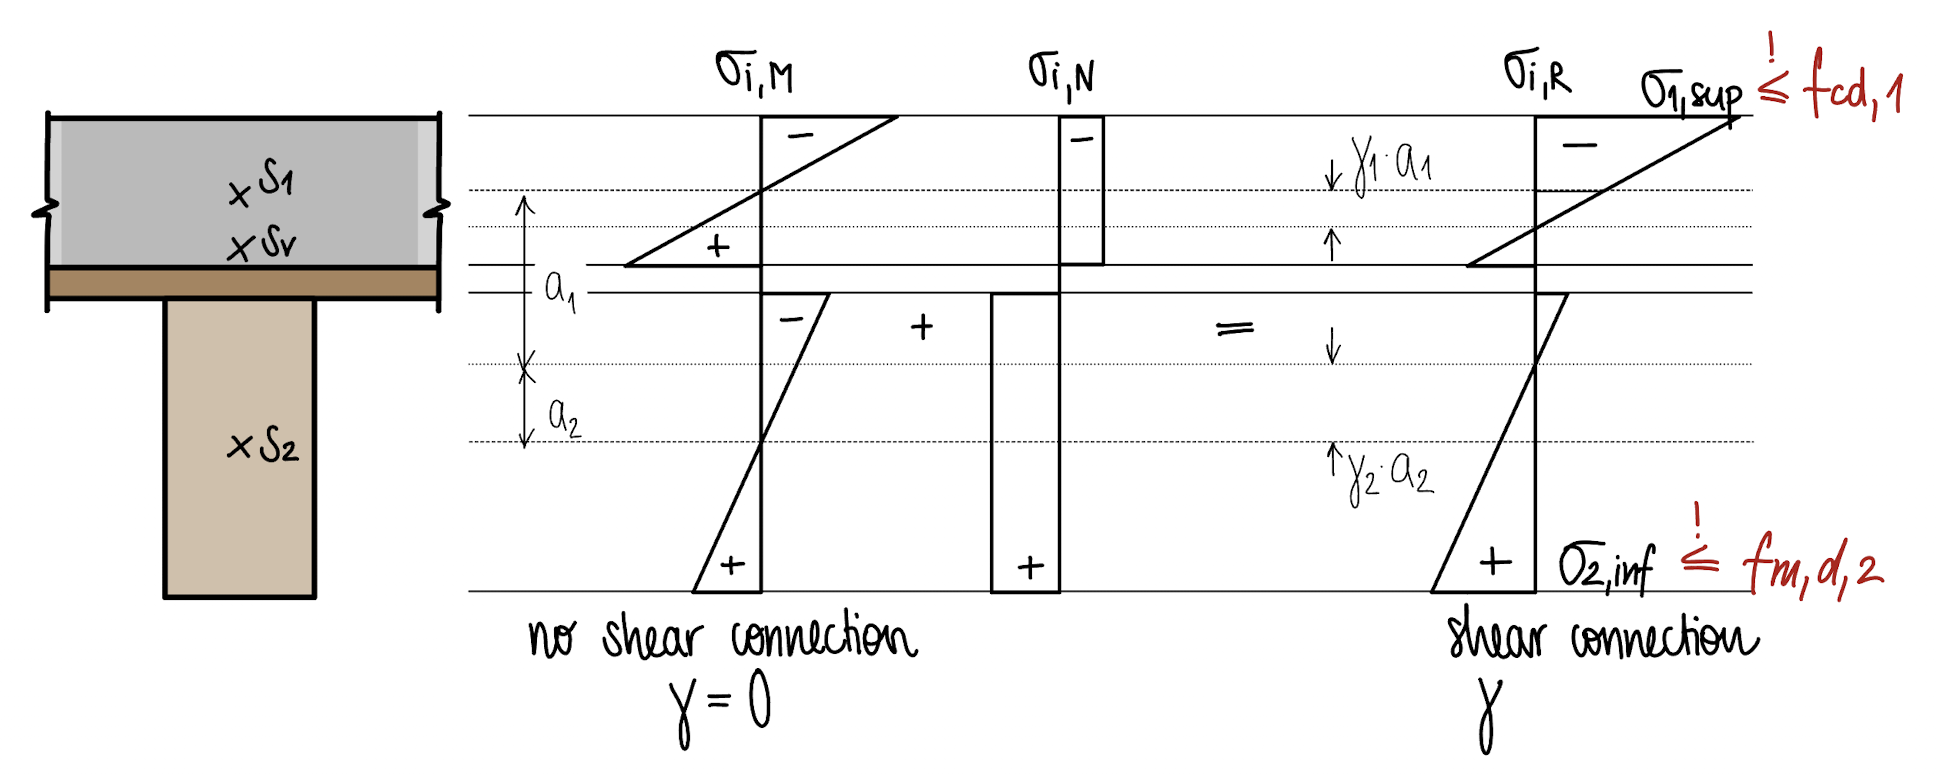
\includegraphics[width=0.9\textwidth]{IMAGES/CS_sigmas.png}
    \caption{Cross-section of a two-layer composite beam with semi-rigid connection according to EN 1995-1-1 \cite{Eurocode5_2023}.}
    \label{fig:composite_section}
\end{figure}

The bending and shear resistances are calculated as
\begin{equation}
\begin{aligned}
m_u
&=
\frac{1}{b}
\min
\left(
f_{cd,1}
\frac{(EI)_{\mathrm{ef}}}{E_1}
\frac{1}{\gamma_1 a_1 + h_1/2},
\;
f_{md,2}
k_{\mathrm{mod}}
\frac{(EI)_{\mathrm{ef}}}{E_2}
\frac{1}{a_2 + h_2/2}
\right),
\\
v_u
&=
\frac{
2 f_{vd,2} k_{\mathrm{mod}}
}
{b}
\frac{(EI)_{\mathrm{ef}}}{E_2}
\frac{1}
     {(a_2+h_2/2)^2}.
\end{aligned}
\end{equation}
The shear resistance is governed by the timber member. For simplification, the shear connection was assumed to be sufficient. Consequently, the detailed design of the connectors was not considered and no connector resistance verification was performed.

\subsubsection{Fire verification}

Fire resistance was evaluated using the residual timber cross-section after charring. A distinction was made between beams exposed on three sides and timber plates exposed on one side. For notched connections, no temperature-dependent reduction in connector stiffness was considered. For screw connectors, the reduction factor $k_{\mathrm{mod,fi}}$ according to Lignum 3.1 was applied \cite{Lignum3.1:2015}.

To satisfy the REI60 requirement, a minimum concrete topping thickness of 80 mm was required \cite{SIA262_2025}. Furthermore, a timber cover of 30 mm was reserved for screw connectors to account for the arrangement of two screws placed side by side.

\subsubsection{Model limitations}

Several simplifications were adopted. The model is limited to one-way structural behaviour and linear-elastic composite action according to the $\gamma$-method. Concrete is assumed to remain uncracked. The shear connection was assumed to provide sufficient resistance. Furthermore, non-linear connector behaviour and differential shrinkage between timber and concrete were not considered.

\subsection{Post-tensioned concrete slab}

Post-tensioned concrete slabs were modelled as flat concrete slabs with unbonded monostrands \cite{Rombach2010, flachdecken_Morgen}. The model extends the reinforced concrete slab formulation by prestressing steel, tendon geometry, load-balancing effects, secondary internal forces, effective bending stiffness, and the additional shear and punching shear resistance provided by tendon deviation forces. The implemented system assumes parabolic tendon profiles. For one-dimensional systems, a distributed tendon layout was assumed. For two-dimensional systems, tendon layouts were represented by distributed and/or banded tendon arrangements, depending on the selected layout configuration.

\subsubsection{Load balancing and tendon geometry}

The post-tensioning force was determined from the load-balancing principle. For a parabolic tendon trajectory, the upward deviation load depends on the prestressing force, tendon eccentricity and span length. For distributed tendons, the equivalent deviation loads in the two orthogonal directions are calculated as

\begin{equation}
u_x
=
\frac{8p_x f_x}{l_x^2},
\qquad
u_y
=
\frac{8p_y f_y}{l_y^2}.
\end{equation}

Here, \(p_x\) and \(p_y\) are the distributed prestressing forces per metre width, \(f_x\) and \(f_y\) are the tendon sag values, and \(l_x\) and \(l_y\) are the corresponding spans. The implemented load-balancing algorithm assigns the required balanced load depending on the selected tendon layout. For distributed tendons in both directions, the structural self-weight is split equally between the two directions and represented by equivalent surface deviation loads. For banded layouts, the tendons are concentrated in the support strips and the internal forces caused by prestressing are derived from equivalent line loads acting along these strips. The prestressing force is selected to balance the structural self-weight estimate available during tendon layout generation.

The tendon profile was defined by the support and mid-span eccentricities. For a parabolic profile,

\begin{equation}
z(x)
=
-\frac{4(e_{\mathrm{span}}-e_{\mathrm{sup}})}{l^2}\,x^2
+
\frac{4(e_{\mathrm{span}}-e_{\mathrm{sup}})}{l}\,x
+
e_{\mathrm{sup}}.
\end{equation}

The eccentricities were selected as the maximum values that satisfy the tendon cover, avoid overlap with the bonded reinforcement and remain within the slab depth. The tendon input values were \(A_p=150\,\mathrm{mm^2}\), \(c_{p,\mathrm{nom}}=30\,\mathrm{mm}\) and \(r_p=6.91\,\mathrm{mm}\).

\subsubsection{Secondary internal forces}

In hyperstatic systems, the deformation caused by post-tensioning is restrained by the supports. This restraint introduces secondary bending moments and secondary shear forces. The total internal forces resulting from the deviation forces of the prestressing system are first calculated using the slab-system coefficients. The secondary internal forces are then obtained by subtracting the primary prestressing contribution:

\begin{equation}
M_{\mathrm{sec}}
=
M_{\mathrm{tot}}(u)
-
P\,e,
\qquad
V_{\mathrm{sec}}
=
V_{\mathrm{tot}}(u)
-
P\,\frac{\partial e}{\partial x}.
\end{equation}

Here, \(M_{\mathrm{tot}}\) and \(V_{\mathrm{tot}}\) denote the total internal forces of the hyperstatic system caused by the deviation forces, \(P\) is the prestressing force and \(e\) is the tendon eccentricity. These secondary internal forces are included in the resistance verification of the post-tensioned slab.

\subsubsection{Effective bending stiffness}

Post-tensioning introduces compressive stresses into the concrete and therefore delays cracking under service loads. For SLS verification, the effective bending stiffness is determined based on the relation between the acting service moment, including secondary moments, and the cracking moment. The cracking moment, initial concrete stress and effective tensile strength are calculated as

\begin{equation}
\begin{aligned}
M_R
&=
\left(
f_{\mathrm{ctm,eff}}
-
\sigma_{c,\mathrm{inf},0}
\right)
\frac{I_I}{h/2},\\
\sigma_{c,\mathrm{inf},0}
&=
-\frac{P}{l\,h}
-
\frac{P\,e_{\max}\,h}{2l\,I_I},\\
f_{\mathrm{ctm,eff}}
&=
\max
\left[
(1.6-h)\,f_{\mathrm{ctm}},
\;
f_{\mathrm{ctm}}
\right].
\end{aligned}
\end{equation}

If the acting service moment does not exceed the cracking moment, the uncracked stiffness is used:

\begin{equation}
(EI)_{\mathrm{eff}}
=
E_{cm}I_I
\qquad
\text{for}
\qquad
\left|M_{\mathrm{Ed,SLS}}+M_{\mathrm{sec}}\right|
\leq
M_R.
\end{equation}

If the cracking moment is exceeded, a partial-cracking factor is calculated and the effective stiffness is interpolated between the uncracked and cracked states as implemented in the code:

\begin{equation}
\begin{aligned}
\zeta
&=
1
-
0.5
\left(
\frac{M_R}{|M_{\mathrm{Ed,SLS}}+M_{\mathrm{sec}}|}
\right)^2,\\
(EI)_{\mathrm{eff}}
&=
\zeta (EI)_I
+
(1-\zeta)(EI)_{II}.
\end{aligned}
\end{equation}

For cracked sections, the local increase of the post-tensioning force is neglected because strain compatibility between concrete and unbonded tendons is not maintained. The cracked neutral-axis depth \(x_{II}\) is obtained from force and moment equilibrium using the effective prestressing force as an external normal force:

\begin{equation}
\begin{aligned}
A_s\sigma_s
+
\frac{P}{l}
&=
\frac{b\,x_{II}}{2}\sigma_{c,\mathrm{inf}},
\\
d_sA_s\sigma_s
+
d_P\frac{P}{l}
+
M_{\mathrm{Ed,SLS}}
+
M_{\mathrm{sec}}
&=
\frac{b\,x_{II}^2}{6}\sigma_{c,\mathrm{inf}}.
\end{aligned}
\end{equation}

The stresses are calculated as

\begin{equation}
\sigma_s
=
\frac{\varepsilon_{c,\mathrm{inf}}}{x_{II}}
(d_s-x_{II})E_s,
\qquad
\sigma_{c,\mathrm{inf}}
=
E_{cm}\varepsilon_{c,\mathrm{inf}}.
\end{equation}

The cracked bending stiffness is calculated from the concrete compression zone and the transformed bonded reinforcement contribution:

\begin{equation}
(EI)_{II}
=
E_{cm}
\left[
\frac{x_{II}^3}{3}
+
\frac{E_s}{E_{cm}}
A_s
(d_s-x_{II})^2
\right].
\end{equation}

The prestressing tendon is not added as a transformed reinforcement area in the cracked inertia because the tendon is unbonded and local strain compatibility is not assumed. Creep is considered in the member deflection calculation through the service load combinations and creep amplification, rather than by reducing \(E_{cm}\) directly in the cracked-section stiffness calculation in accordance with the existing rectangular concrete handling.

\subsubsection{Bending and one-way shear resistance}

The bending resistance accounts for the contribution of the prestressing steel and the bonded reinforcement. The design bending moment includes the effects of external loads and secondary moments:

\begin{equation}
M_d
=
M_{g,d}
+
M_{q,d}
+
M_{\mathrm{sec}}
\leq
M_{Rd}.
\end{equation}

The bending resistance and the corresponding compression-zone depth are calculated as

\begin{equation}
\begin{aligned}
M_{Rd}
&=
\frac{P}{l}
\left(
d_P-\frac{0.85x}{2}
\right)
+
A_s f_{sd}
\left(
d_s-\frac{0.85x}{2}
\right),
\\
x
&=
\frac{
A_s f_{sd}
+
P/l
}
{
b_{\mathrm{eff}} f_{cd}
}.
\end{aligned}
\end{equation}

Ductility is ensured by limiting the compression-zone depth and by providing minimum bonded reinforcement. For the minimum bonded reinforcement check, the ordinary reinforced-concrete cracking moment is used, while the prestress-increased cracking moment is used for serviceability stiffness.

For systems without column supports, one-way shear is checked. The design shear force includes the secondary shear force and is verified against the concrete shear resistance and the vertical component of the prestressing force:

\begin{equation}
\begin{aligned}
V_d
&=
V_{g,d}
+
V_{q,d}
+
V_{\mathrm{sec}}
\leq
V_{Rd}
+
P_{\infty}\sin(\beta_P),\\
\sin(\beta_P)
&=
\frac{4f}{L}.
\end{aligned}
\end{equation}

Here, \(V_{Rd}\) is calculated according to the reinforced concrete shear resistance model of the rectangular concrete section. The post-tensioning contribution is added through the vertical component of the prestressing force.

\subsubsection{Punching shear resistance}

For slabs supported by columns, punching shear is checked instead of one-way shear. The concrete punching resistance without punching reinforcement is implemented as level of approximation 2 \cite{SIA262_2025}:

\begin{equation}
\begin{aligned}
V_{Rd,c}(\psi)
&=
k_r\,\tau_{cd}\,d_v\,u,
\\
k_r
&=
\frac{1}
{
0.45
+
0.18\,\psi\,d_v\,k_g
}
\leq
2,
\qquad
k_g
=
\frac{48}
{16+D_{\max}}.
\end{aligned}
\end{equation}

The slab rotation is calculated as

\begin{equation}
\begin{aligned}
\psi
&=
1.5
\frac{r_s}{d_v}
\frac{f_{sd}}{E_s}
\left(
\frac{m_{sd}}{m_{Rd}}
\right)^{3/2},\\
r_s &= 0.22l.
\end{aligned}
\end{equation}

The rotation is determined independently for both orthogonal directions, and the larger value governs:

\begin{equation}
\psi
=
\max(\psi_x,\psi_y).
\end{equation}

The design action is calculated as

\begin{equation}
V_{Ed}
=
V_{g,d}
+
V_{q,d}
+
V_{\mathrm{sec}},
\end{equation}

where \(V_{\mathrm{sec}}\) is the secondary shear force caused by restraint of the prestressing deformation. Without punching reinforcement, the verification is

\begin{equation}
V_{Ed}
\leq
V_{Rd,c}(\psi).
\end{equation}

For post-tensioned slabs, the resistance is increased by the vertical component of the prestressing force above the column:

\begin{equation}
V_{Rd,\mathrm{punch}}
=
V_{Rd,c}(\psi)
+
V_{P,\mathrm{punch}}.
\end{equation}

The prestressing contribution is calculated from the support-strip tendons and the distributed tendons crossing the control width around the column:

\begin{equation}
V_{P,\mathrm{punch}}
=
\left(
P_{sx,\infty}
+
p_{dx,\infty} b_{0,y}
\right)
\sin(\beta_{P,x})
+
\left(
P_{sy,\infty}
+
p_{dy,\infty} b_{0,x}
\right)
\sin(\beta_{P,y}).
\end{equation}

The forces \(P_{sx}\) and \(P_{sy}\) are the post-tensioning forces in the support strips and are assumed to act fully over the column. Distributed tendons are only considered over the relevant control width around the column.

If punching reinforcement is required, the existing shear reinforcement definition of the cross-section is used for the resistance calculation. No separate punching reinforcement object is introduced in the structural model. For material accounting in the final comparison, required punching reinforcement is post-processed as an additional averaged steel quantity. The resistance is calculated as

\begin{equation}
V_{Rd,\mathrm{punch}}
=
V_{Rd,c}(\psi)
+
V_{Rd,s}
+
V_{P,\mathrm{punch}},
\end{equation}

with an upper limit applied to the sum of concrete and punching reinforcement resistance in the implementation.

\subsubsection{Model limitations}

Several simplifications were adopted. The model is limited to unbonded monostrands with parabolic tendon profiles. Friction losses were neglected. Local anchorage verification and local concrete crushing at anchorages were not considered. For cracked sections, the local increase in prestressing force is neglected because strain compatibility is not maintained for unbonded tendons. The model also assumes that the selected prestressing layout can be arranged within the geometric constraints of the slab and anchorage system. The effective stiffness model is a simplified post-processing approach and does not include a transformed unbonded tendon contribution in the cracked inertia.

\subsection{Automated acoustic floor build-up generator \label{Sec: AutFloor}}

The generator enables floor build-up handling dependent on the structural cross-section. It adds the lightest non-structural floor build-up that satisfies the selected airborne and impact sound targets. The purpose is to compare slab systems on the basis of complete floor assemblies rather than structural cross-sections only. The generator distinguishes between normal and increased acoustic requirements according to SIA 181 \cite{SIA181_2020}. The target values are summarised in Table~\ref{Tab: ReqSS}.

The workflow of the generator is shown in Figure~\ref{fig:acoustic_floor_generator}. First, the structural cross-section is converted into an area-related mass. Airborne sound insulation and impact sound level are then estimated with the mass-law relationship \cite{BauphysikKalender, ISO12354_1_2017, ISO12354_2_2017}:

\begin{equation}
\begin{aligned}
R_{w,\mathrm{mass}} &= 37.5 \log_{10}(m'_{\mathrm{base}}) - 42,\\
L_{n,w,\mathrm{mass}} &= 164 - 35 \log_{10}(m'_{\mathrm{base}}).
\end{aligned}
\end{equation}

If the bare structural cross-section does not fulfil the acoustic targets, a floating floor consisting of glass wool, cement screed and parquet is added. Screed thicknesses of 60 mm and 85 mm are checked first. The floating floor is represented by a simplified mass-spring-mass model \cite{BauphysikKalender, ISO12354_1_2017, ISO12354_2_2017}:

\begin{equation}
\begin{aligned}
(s'_{\mathrm{eff}})^{-1}
&=
\sum_i (s'_i)^{-1},\\
f_{0,R} &=
\frac{1}{2\pi}
\sqrt{
s'_{\mathrm{eff}}\,10^6
\left(
\frac{1}{m'_{\mathrm{base}}}
+
\frac{1}{m'_{\mathrm{screed}}}
\right)
},\\
\Delta R_{w,\mathrm{fl}} &=
74.4 - 20\log_{10}(f_{0,R}) - \frac{R_{w,\mathrm{mass}}}{2},\\
f_{0,L} &=
160\sqrt{\frac{s'_{\mathrm{eff}}}{m'_{\mathrm{screed}}}},\\
\Delta L_{n,w,\mathrm{fl}} &=
\operatorname{mean}_{f_i \leq f_{\max}}
\left[
30\log_{10}
\left(
\frac{f_i}{f_{0,L}}
\right)
\right].
\end{aligned}
\end{equation}

Here, \(s'_{\mathrm{eff}}\) is the effective dynamic stiffness of the glass-wool layer in \(\mathrm{MN/m^3}\). For TCC sections with two insulation layers, the layers are treated as springs in series.

If the acoustic targets are still not met, gravel is added below the spring layer in discrete steps. TCC sections use a separate branch because the concrete topping is already part of the structural cross-section. The concrete layer is therefore treated as mass and impact damping, and no additional gravel is generated. Gravel, hollow-core insulation and the TCC concrete topping all use damping corrections \cite{BauphysikKalender}.

\begin{figure}[htbp]
\centering
\resizebox{\textwidth}{!}{%
    \begin{tikzpicture}[
    font=\small,
    >=Latex,
    arrow/.style={->, thick},
    box/.style={draw, rounded corners=1pt, align=center, minimum width=3.2cm, minimum height=1.0cm},
    widebox/.style={draw, rounded corners=1pt, align=center, minimum width=4.4cm, minimum height=1.12cm},
    eqbox/.style={draw, rounded corners=1pt, align=center, minimum width=5.1cm, minimum height=1.35cm},
    corrbox/.style={draw, rounded corners=1pt, align=center, minimum width=6.1cm, minimum height=1.8cm}
]

\node[box] (section) at (0,0) {Structural\\cross-section};
\node[eqbox] (mass) at (4.7,0) {Mass law\\[-1pt]
    \(m'_{\mathrm{base}}\)\\[1pt]
    \(R_{w,\mathrm{mass}}, L_{n,w,\mathrm{mass}}\)};
\node[box] (checkbare) at (9.5,0) {Targets\\fulfilled?};
\node[box] (none) at (13.9,1.65) {No additional\\floor build-up};
\node[widebox] (floating) at (13.9,-1.65) {Floating floor\\glass wool + screed + parquet};
\node[eqbox] (spring) at (19.3,-1.65) {Mass-spring-mass\\[-1pt]
    \(f_{0,R}, f_{0,L}\)\\[1pt]
    \(\Delta R_{w,\mathrm{fl}},\Delta L_{n,w,\mathrm{fl}}\)};
\node[corrbox] (damping) at (25.4,-1.65) {Damping corrections\\[-1pt]
    gravel: \(\Delta_{\mathrm{gravel}}\leq6\,\mathrm{dB}\)\\[-1pt]
    hollow-core: \(\Delta_{\mathrm{hc}}=\min(6h_{\mathrm{ins}}/0.20,7)\)\\[-1pt]
    TCC topping: \(\Delta_{\mathrm{tcc}}\leq6\,\mathrm{dB}\)};
\node[widebox] (tcc) at (19.3,-3.75) {TCC branch\\topping as mass\\and impact damping};
\node[eqbox] (output) at (32.0,0) {Complete floor assembly\\[-1pt]
    \(R_w=R_{w,\mathrm{mass}}+\Delta R\)\\[1pt]
    \(L_{n,w}=L_{n,w,\mathrm{mass}}-\Delta L\)};

\draw[arrow] (section) -- (mass);
\draw[arrow] (mass) -- (checkbare);
\draw[arrow] (checkbare) -- node[above, font=\small] {yes} (none);
\draw[arrow] (checkbare) -- node[below, font=\small] {no} (floating);
\draw[arrow] (floating) -- (spring);
\draw[arrow] (spring) -- (damping);
\draw[arrow] (floating) -- (tcc);
\draw[arrow] (none) -| (output);
\draw[arrow] (damping) -| (output);
\draw[arrow] (tcc) -| (damping);

\end{tikzpicture}

}
\caption{Workflow of the automated acoustic floor build-up generator.}
\label{fig:acoustic_floor_generator}
\end{figure}

The implemented acoustic model is intentionally simplified. A fully spectral prediction would require measured $R(f)$, $L_n(f)$ and $\Delta L(f)$ data for every structural system and floor layer. Such data is not available consistently for all systems in the optimisation. Thus, the model averages across the calculated frequencies. The selected model is therefore used as a robust comparative approximation, not as a replacement for project-specific acoustic verification.

\subsection{Final comparison setup}

The final comparison was defined through a set of residential and office cases with fixed load levels, discrete span values, structural systems and material groups. The cases are summarised in Table~\ref{tab:final_comparison_cases}. The corresponding start values, optimisation variables and bounds are listed in Table~\ref{tab:final_comparison_bounds}. This separation keeps the comparison inputs transparent: Table~\ref{tab:final_comparison_cases} defines which systems are compared, while Table~\ref{tab:final_comparison_bounds} defines how each system is optimised.

\begin{table*}[t]
    \centering
    \begingroup
    \scriptsize
    \setlength{\tabcolsep}{3.5pt}
    \renewcommand{\arraystretch}{1.2}
    \begin{tabularx}{\textwidth}{@{}l|c|l|>{\hsize=0.7\hsize\raggedright\arraybackslash}X|>{\hsize=0.7\hsize\raggedright\arraybackslash}X|>{\hsize=0.8\hsize\raggedright\arraybackslash}X|>{\hsize=1.8\hsize\raggedright\arraybackslash}X@{}}
    \hline
    \textbf{Case} &
    \textbf{$q_k$} &
    \textbf{Span} &
    \textbf{Cross-section} &
    \textbf{Description} &
    \textbf{Structural system} &
    \textbf{Materials / fixed input} \\
    & kN/m$^2$ & m & & & & \\ \hline
    Residential & 2.0 & 3, 5, 6, 7, 8, 10 &
    Rectangular concrete &
    conventionally reinforced &
    2-way, full continuity, walls &
    ready-mixed concrete, B500B; fixed line supports \\

    Residential & 2.0 & 3, 5, 6, 7, 8, 10 &
    Rectangular concrete PT &
    post-tensioned, distributed layout &
    2-way, full continuity, walls &
    ready-mixed concrete, B500B, Y1860; layout $[0,1,0,1]$; fixed line supports\\

    Residential & 2.0 & 3, 5, 6, 7, 8, 10 &
    Rectangular wood &
    BSH &
    Simple span &
    glue-laminated timber and solid structural timber; fire from bottom \\

    Residential & 2.0 & 3, 5, 6, 7, 8, 10 &
    TCC &
    BSH, kerve, $s=0.50$\,m &
    Simple span &
    ready-mixed concrete, B500B, BSH, kerve; $a_{\mathrm{ribs}}=1.00$\,m, $b_w=1.00$\,m \\

    Residential & 2.0 & 3, 5, 6, 7, 8, 10 &
    TCC &
    ribs, DBS\_10, $s=0.06$\,m (2 rows $s=0.12$\,m) &
    Simple span &
    ready-mixed concrete, B500B, BSH, DBS\_10; $a_{\mathrm{ribs}}=0.625$\,m, $b_w=0.18$\,m \\

    Residential & 2.0 & 3, 5, 6, 7, 8, 10 &
    Ribbed timber &
    hollow-core &
    Simple span &
    glue-laminated timber and solid structural timber; fire from bottom and sides \\

    Office & 3.0 & 8, 10, 12, 16 &
    Rectangular concrete &
    conventionally reinforced &
    2-way, full continuity, columns &
    ready-mixed concrete, B500B; fixed point supports \\

    Office & 3.0 & 8, 10, 12, 16 &
    Rectangular concrete PT &
    post-tensioned, distributed layout &
    2-way, full continuity, columns &
    ready-mixed concrete, B500B, Y1860; layout $[0,1,0,1]$; fixed point supports \\

    Office & 3.0 & 8, 10, 12, 16 &
    Rectangular concrete PT &
    post-tensioned, banded layout &
    2-way, full continuity, columns &
    ready-mixed concrete, B500B, Y1860; layout $[1,0,1,0]$; fixed point supports \\

    Office & 3.0 & 8, 10, 12, 16 &
    Ribbed concrete &
    conventionally reinforced &
    Continuous beam &
    ready-mixed concrete, B500B; fire from bottom and sides \\

    \hline
    \end{tabularx}
    \endgroup
    \caption{Input definition for the final comparison of slab systems. Only the discrete span values available in \texttt{slab\_properties.db} are used. The listed material groups are taken from \texttt{database\_260126.db}; for each mechanical property, the dataset generator considers the best and worst available EPD by GWP.}
    \label{tab:final_comparison_cases}
\end{table*}

\begin{table*}[t]
    \centering
    \begingroup
    \scriptsize
    \setlength{\tabcolsep}{4pt}
    \renewcommand{\arraystretch}{1.2}
    \begin{tabularx}{\textwidth}{@{}l|>{\hsize=0.7\hsize\raggedright\arraybackslash}X|l|>{\hsize=1.3\hsize\raggedright\arraybackslash}X@{}}
    \hline
    \textbf{Cross-section} &
    \textbf{Start values} &
    \textbf{Optimisation variables} &
    \textbf{Bounds / fixed values} \\ \hline

    Rectangular concrete 2D &
    $b=1.00$\,m, $h=0.20$\,m generally; office start heights $h_0=\{0.25,0.35,0.45,0.60\}$\,m for $l=\{8,10,12,16\}$\,m &
    $h$, $\varnothing_{xu}$, $\varnothing_{xo}$, $\varnothing_w$ &
    $h=0.16$--$1.20$\,m, $\varnothing_{xu/xo}=6$--$40$\,mm, $\varnothing_w=0$--$20$\,mm; $s=0.15$\,m; y-reinforcement follows x-reinforcement \\

    Rectangular concrete PT 2D &
    $b=1.00$\,m, $h=0.20$\,m generally; office start heights $h_0=\{0.20,0.25,0.30,0.40\}$\,m for $l=\{8,10,12,16\}$\,m &
    $h$, $\varnothing_{xu}$, $\varnothing_{xo}$, $\varnothing_w$ &
    $h=0.18$--$1.20$\,m, $\varnothing_{xu/xo}=6$--$40$\,mm, $\varnothing_w=0$--$20$\,mm; $s=0.15$\,m; Y1860 monostrands; load balancing from PT layout \\

    Rectangular wood 1D &
    $b=1.00$\,m, $h=0.10$\,m &
    $h$ &
    section height optimised for the governing criterion; glue-laminated timber and solid structural timber variations from database \\

    Ribbed timber 1D &
    $b=0.12$\,m, $h=0.22$\,m, $a=0.625$\,m, $t_2=25$\,mm, $t_3=27$\,mm &
    $b$, $h$, $t_2$, $t_3$ &
    $b=0.10$--$0.24$\,m, $h=0.22$--$2.00$\,m, $t_2=25$--$160$\,mm, $t_3=27$--$160$\,mm; rib spacing fixed at $a=0.625$\,m \\

    Ribbed concrete 1D &
    $b=1.00$\,m, $b_w=0.25$\,m, $h=0.30$\,m, $h_f=0.18$\,m &
    $h_w$, $h_f$, $\varnothing_{x,w}$, $b_w$, $b$ &
    $h_w=0.04$--$2.00$\,m, $h_f=0.08$--$0.50$\,m in 1D / $0.12$--$0.50$\,m in 2D optimiser, $\varnothing_{x,w}=8$--$40$\,mm, $b_w=0.15$--$0.40$\,m, $b=0.40$--$2.50$\,m \\

    TCC 1D &
    Residential: $h_c=0.08$\,m, $h_w=0.12$\,m; office TCC starts $(h_c/h_w)=0.12/0.30$, $0.16/0.35$, $0.20/0.40$, $0.25/0.70$\,m for $l=8$, 10, 12, 16\,m &
    $h_c$, $h_w$ &
    $h_c=0.08$--$0.50$\,m, $h_w=0.08$--$1.50$\,m; flat residential $s=0.50$\,m; ribbed residential $s=0.15$\,m, $b_w=0.18$\,m; ribbed office $s=0.06$\,m, $b_w=0.24$\,m \\ \hline
    \end{tabularx}
    \endgroup
    \caption{Start values, optimisation variables and bounds used for the final comparison. All systems are optimised for GWP with $n_{\mathrm{iter}}=150$; the automated acoustic floor build-up is enabled with normal acoustic requirements. Material variations are generated from the EPD best and worst cases within each mechanical property class.}
    \label{tab:final_comparison_bounds}
\end{table*}

\subsubsection{Sampling of material variants}

In the final comparison, material variation is generated by selecting the best and worst available EPD by GWP within each mechanical property group. Thus, for example, concrete strength class C30/37 is sampled with its lowest and highest available product-specific GWP, but it is not mixed with another strength class.

\subsection{Verification of implemented models}

\subsubsection{Timber--concrete composite slab}

The implementation of the $\gamma$-method was verified against a hand calculation based on a representative timber--concrete composite floor system. The selected geometry, material properties and connector configuration corresponded to a typical residential floor. The verification focused on the effective bending stiffness, as this quantity governs both resistance and serviceability calculations.

The verification model used the following set-up:

\begin{itemize}
    \item Concrete C30/37: $h_c = 0.080\,\mathrm{m}$, $b_{\mathrm{ef}} = 0.60\,\mathrm{m}$, $A_c = 0.048\,\mathrm{m}^2$, $I_c = 2.56 \times 10^{-5}\,\mathrm{m}^4$, $E_{cm} = 34\,\mathrm{GPa}$, $\varphi_c = 2.5$.
    
    \item Timber ribs GL24h: $a_{\mathrm{ribs}} = 0.6\,\mathrm{m}$, $h_w = 0.241\,\mathrm{m}$, $b_w = 0.12\,\mathrm{m}$, $A_w = 0.0289\,\mathrm{m}^2$, $I_w = 1.399 \times 10^{-4}\,\mathrm{m}^4$, $E_{w,\mathrm{mean}} = 11.5\,\mathrm{GPa}$, $d = 0.02\,\mathrm{m}$, $k_{\mathrm{def}} = 0.6$.
    
    \item Connection DBS\_10: $s = 0.25\,\mathrm{m}$, $K_{\mathrm{ser}} = 9.7\,\mathrm{MN/m}$, $k'_{\mathrm{def}} = 1.2$.
    
    \item Structural system: single-span system with $l_0 = 6.0\,\mathrm{m}$.
\end{itemize}


Table~\ref{tab:TCCVer} summarises the calculated $\gamma_c$ factors, the lever arms to the neutral axis ($a_c$ and $a_w$), and the resulting effective bending stiffness per metre width. The comparison showed excellent agreement between the manual calculations and the implementation. The maximum deviation remained below $0.2\,\%$, confirming the correct implementation of the $\gamma$-method across the time-dependent stiffness calculations.

\begin{table}[h!]
    \centering
    \begingroup
    \scriptsize
    \setlength{\tabcolsep}{3pt}
    \renewcommand{\arraystretch}{1.12}
    \begin{tabularx}{\textwidth}{@{}l|c|c|c|c|r|r@{}}
    \hline
    \textbf{Case} &
    \textbf{Time} &
    $\gamma_c$ &
    $a_c$ [m] &
    $a_w$ [m] &
    $EI_{\mathrm{eff,manual}}$ [$\mathrm{kN\,m^2/m}$] &
    $EI_{\mathrm{eff,test}}$ [$\mathrm{kN\,m^2/m}$] \\
    \hline
    SLS & $t=0$       & 0.0798 & 0.1299 & 0.0508 & 9225.00 & 9238.66 \\
    SLS & $t=\infty$ & 0.2279 & 0.1459 & 0.0348 & 4053.00 & 4059.49 \\
    ULS & $t=0$       & 0.0547 & 0.1425 & 0.0382 & 7962.00 & 7972.65 \\
    ULS & $t=\infty$ & 0.1645 & 0.1541 & 0.0265 & 3537.00 & 3540.68 \\
    \hline
    \end{tabularx}
    \endgroup
    \caption{Comparison of manual calculations to test-case output for effective bending stiffness values in $\mathrm{kN\,m^2/m}$.}
    \label{tab:TCCVer}
\end{table}

\subsubsection{Post-tensioned concrete slab}

The implementation of the post-tensioned slab class was checked using a diagnostic test file with a fixed set-up. The verification case covers the bending resistance and the quasi-permanent deflection of a two-way post-tensioned slab with distributed tendons and wall supports.

The verification model used the following set-up:

\begin{itemize}
    \item Materials: concrete C30/37, reinforcing steel B500B, prestressing steel Y1860.
    \item Structural system: two-way slab with wall supports and \(l_x=l_y=6.0\,\mathrm{m}\).
    \item Geometry: slab thickness \(h=280\,\mathrm{mm}\), effective depth of bonded steel \(d_s\), and effective depth of prestressing steel \(d_P\) as calculated from the reinforcement and tendon cover constraints.
    \item Tendon layout: distributed
    \item Loads: \(g_{0,k}\), \(g_{2,k}=0.75\,\mathrm{kN/m^2}\), \(q_k=2.00\,\mathrm{kN/m^2}\),  \(\varphi=2.0\).
\end{itemize}

The bending resistance was calculated from the contribution of the prestressing steel and the bonded reinforcement:

\begin{equation}
    M_{Rd}
    =
    \frac{P_{\infty}}{l}
    \left(d_p-\frac{0.85x}{2}\right)
    +
    A_s f_{sd}
    \left(d_s-\frac{0.85x}{2}\right)
\end{equation}

\begin{equation}
\begin{aligned}
x
&=
\frac{\frac{P_{\infty}}{l}+A_s f_{sd}}
{b f_{cd}},\\
\frac{P_{\infty}}{l}
&=
76.39\,\mathrm{kN/m},\\
A_s
&=
\frac{\pi \cdot 14^2}{4 \cdot 150}
=
1026\,\mathrm{mm^2/m},\\
f_{sd} &= 435\,\mathrm{MPa},
\qquad
f_{pd}=1391\,\mathrm{MPa},\\
x &= 31.36\,\mathrm{mm},
\qquad
0.85x=26.65\,\mathrm{mm}.
\end{aligned}
\end{equation}

The prestressing and bonded reinforcement contributions are

\begin{equation}
\begin{aligned}
M_{Rd,p}
&=
76.39
\left(
0.2431-\frac{0.02665}{2}
\right)
=
17.55\,\mathrm{kNm/m},\\
M_{Rd,s}
&=
1026 \cdot 10^{-6}
\cdot 435000
\left(
0.253-\frac{0.02665}{2}
\right)
=
106.94\,\mathrm{kNm/m},\\
M_{Rd}
&=
17.55+106.94
=
124.49\,\mathrm{kNm/m}.
\end{aligned}
\end{equation}

\paragraph{Deflection calculation}

The quasi-permanent load combination, the net load after load balancing and the long-term reference deflection are

\begin{equation}
\begin{aligned}
q_{\mathrm{per}}
&=
g_{0,k}+g_{1,k}+g_{2,k}+\psi_2 q_k
=
7.00+0.00+0.75+0.30\cdot2.00
=
8.35\,\mathrm{kN/m^2},\\
g_{0,k}
&=
7.00\,\mathrm{kN/m^2},\\
q_{\mathrm{net}}
&=
q_{\mathrm{per}}-g_{0,k}
=
1.35\,\mathrm{kN/m^2}.
\end{aligned}
\end{equation}

In Cubus Cedrus the same action was applied with the corresponding sign convention. The uncracked elastic deflection and long-term deflection are

\begin{equation}
\begin{aligned}
q_{\mathrm{net,Cedrus}}
&=
-1.350\,\mathrm{kN/m^2},\\
w_{\mathrm{Cedrus},\varphi=0}
&=
0.0349\,\mathrm{mm},\\
w_{\varphi}
&=
w_{\varphi=0}(1+\varphi),\\
w_{\mathrm{Cedrus},\varphi=2.0}
&=
0.0349\cdot3
=
0.1047\,\mathrm{mm}.
\end{aligned}
\end{equation}


The hand calculation is compared with the output of \inlinecode{test\_pt\_2D.py}.

\begin{table}[H]
    \centering
    \begingroup
    \scriptsize
    \setlength{\tabcolsep}{3pt}
    \renewcommand{\arraystretch}{1.12}
    \begin{tabularx}{0.65\textwidth}{@{}l|r|r|r@{}}
    \hline
    \textbf{Result} & \textbf{Calculation} & \textbf{Python} & \textbf{Difference} \\
    \hline
    $M_{Rd}$ & $124.49$ & $124.49$ & $0.0\%$ \\
    $M_{cr,PT}$ & $100.83$ & $100.83$ & $0.0\%$ \\
    $w_{\varphi=2.0}$ & $0.1047$ & $0.1037$ & $-1.0\%$ \\
    \hline
    \end{tabularx}
    \endgroup
    \caption{Validation of bending resistance and quasi-permanent deflection. $M$ values are given in $\mathrm{kNm/m}$ and deflections in $\mathrm{mm}$.}
    \label{tab:pt_verification_methods}
\end{table}

The bending resistance fulfils the minimum bonded reinforcement condition:

\begin{equation}
    M_{Rd}
    =
    124.49\,\mathrm{kNm/m}
    >
    M_{cr,PT}
    =
    100.83\,\mathrm{kNm/m}
\end{equation}

The calculated long-term deflection agrees with the Cedrus reference value. The small difference results from rounding of the printed deflection and material parameters.
